% Created by tikzDevice version 0.10.1 on 2017-12-04 16:18:48
% !TEX encoding = UTF-8 Unicode
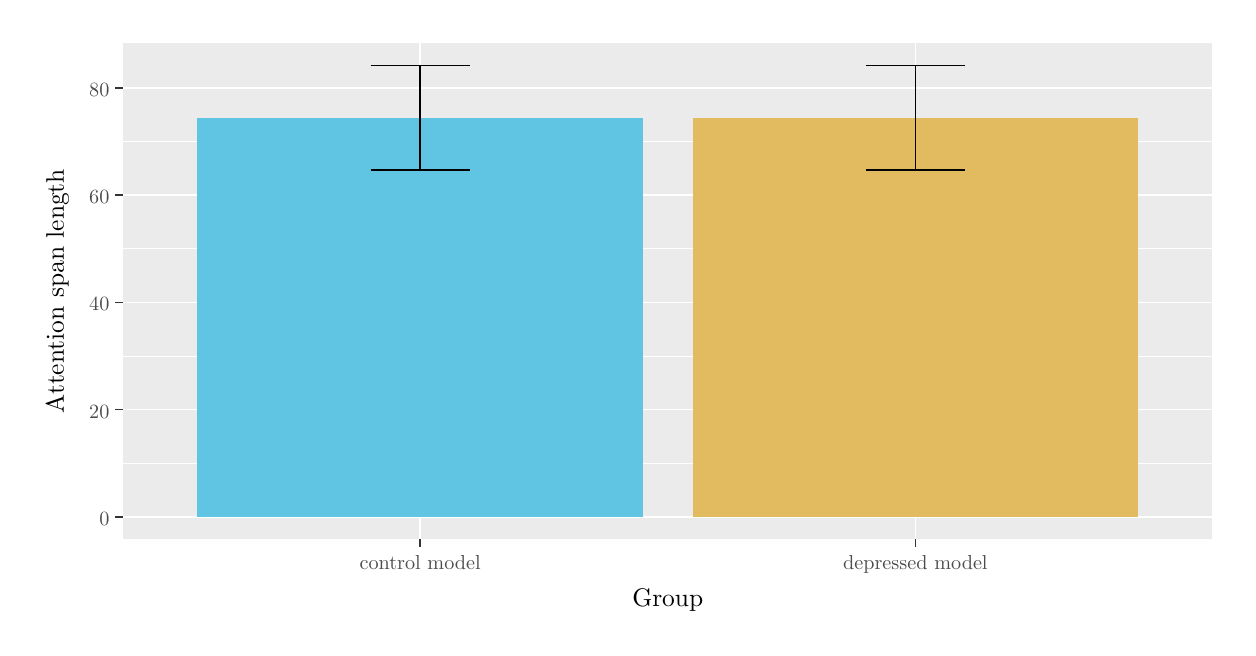
\begin{tikzpicture}[x=1pt,y=1pt]
\definecolor{fillColor}{RGB}{255,255,255}
\path[use as bounding box,fill=fillColor,fill opacity=0.00] (0,0) rectangle (433.62,216.81);
\begin{scope}
\path[clip] (  0.00,  0.00) rectangle (433.62,216.81);
\definecolor{drawColor}{RGB}{255,255,255}
\definecolor{fillColor}{RGB}{255,255,255}

\path[draw=drawColor,line width= 0.6pt,line join=round,line cap=round,fill=fillColor] (  0.00,  0.00) rectangle (433.62,216.81);
\end{scope}
\begin{scope}
\path[clip] ( 34.47, 31.92) rectangle (428.12,211.31);
\definecolor{fillColor}{gray}{0.92}

\path[fill=fillColor] ( 34.47, 31.92) rectangle (428.12,211.31);
\definecolor{drawColor}{RGB}{255,255,255}

\path[draw=drawColor,line width= 0.3pt,line join=round] ( 34.47, 59.43) --
	(428.12, 59.43);

\path[draw=drawColor,line width= 0.3pt,line join=round] ( 34.47, 98.15) --
	(428.12, 98.15);

\path[draw=drawColor,line width= 0.3pt,line join=round] ( 34.47,136.88) --
	(428.12,136.88);

\path[draw=drawColor,line width= 0.3pt,line join=round] ( 34.47,175.60) --
	(428.12,175.60);

\path[draw=drawColor,line width= 0.6pt,line join=round] ( 34.47, 40.07) --
	(428.12, 40.07);

\path[draw=drawColor,line width= 0.6pt,line join=round] ( 34.47, 78.79) --
	(428.12, 78.79);

\path[draw=drawColor,line width= 0.6pt,line join=round] ( 34.47,117.51) --
	(428.12,117.51);

\path[draw=drawColor,line width= 0.6pt,line join=round] ( 34.47,156.24) --
	(428.12,156.24);

\path[draw=drawColor,line width= 0.6pt,line join=round] ( 34.47,194.96) --
	(428.12,194.96);

\path[draw=drawColor,line width= 0.6pt,line join=round] (141.83, 31.92) --
	(141.83,211.31);

\path[draw=drawColor,line width= 0.6pt,line join=round] (320.76, 31.92) --
	(320.76,211.31);
\definecolor{fillColor}{RGB}{95,197,226}

\path[fill=fillColor] ( 61.31, 40.07) rectangle (222.35,184.31);
\definecolor{fillColor}{RGB}{226,186,95}

\path[fill=fillColor] (240.24, 40.07) rectangle (401.28,184.31);
\definecolor{drawColor}{RGB}{0,0,0}

\path[draw=drawColor,line width= 0.6pt,line join=round] (123.94,203.16) --
	(159.72,203.16);

\path[draw=drawColor,line width= 0.6pt,line join=round] (141.83,203.16) --
	(141.83,165.46);

\path[draw=drawColor,line width= 0.6pt,line join=round] (123.94,165.46) --
	(159.72,165.46);

\path[draw=drawColor,line width= 0.6pt,line join=round] (302.87,203.16) --
	(338.65,203.16);

\path[draw=drawColor,line width= 0.6pt,line join=round] (320.76,203.16) --
	(320.76,165.46);

\path[draw=drawColor,line width= 0.6pt,line join=round] (302.87,165.46) --
	(338.65,165.46);
\end{scope}
\begin{scope}
\path[clip] (  0.00,  0.00) rectangle (433.62,216.81);
\definecolor{drawColor}{gray}{0.30}

\node[text=drawColor,anchor=base east,inner sep=0pt, outer sep=0pt, scale=  0.73] at ( 29.52, 37.04) {0};

\node[text=drawColor,anchor=base east,inner sep=0pt, outer sep=0pt, scale=  0.73] at ( 29.52, 75.76) {20};

\node[text=drawColor,anchor=base east,inner sep=0pt, outer sep=0pt, scale=  0.73] at ( 29.52,114.48) {40};

\node[text=drawColor,anchor=base east,inner sep=0pt, outer sep=0pt, scale=  0.73] at ( 29.52,153.21) {60};

\node[text=drawColor,anchor=base east,inner sep=0pt, outer sep=0pt, scale=  0.73] at ( 29.52,191.93) {80};
\end{scope}
\begin{scope}
\path[clip] (  0.00,  0.00) rectangle (433.62,216.81);
\definecolor{drawColor}{gray}{0.20}

\path[draw=drawColor,line width= 0.6pt,line join=round] ( 31.72, 40.07) --
	( 34.47, 40.07);

\path[draw=drawColor,line width= 0.6pt,line join=round] ( 31.72, 78.79) --
	( 34.47, 78.79);

\path[draw=drawColor,line width= 0.6pt,line join=round] ( 31.72,117.51) --
	( 34.47,117.51);

\path[draw=drawColor,line width= 0.6pt,line join=round] ( 31.72,156.24) --
	( 34.47,156.24);

\path[draw=drawColor,line width= 0.6pt,line join=round] ( 31.72,194.96) --
	( 34.47,194.96);
\end{scope}
\begin{scope}
\path[clip] (  0.00,  0.00) rectangle (433.62,216.81);
\definecolor{drawColor}{gray}{0.20}

\path[draw=drawColor,line width= 0.6pt,line join=round] (141.83, 29.17) --
	(141.83, 31.92);

\path[draw=drawColor,line width= 0.6pt,line join=round] (320.76, 29.17) --
	(320.76, 31.92);
\end{scope}
\begin{scope}
\path[clip] (  0.00,  0.00) rectangle (433.62,216.81);
\definecolor{drawColor}{gray}{0.30}

\node[text=drawColor,anchor=base,inner sep=0pt, outer sep=0pt, scale=  0.73] at (141.83, 20.91) {control model};

\node[text=drawColor,anchor=base,inner sep=0pt, outer sep=0pt, scale=  0.73] at (320.76, 20.91) {depressed model};
\end{scope}
\begin{scope}
\path[clip] (  0.00,  0.00) rectangle (433.62,216.81);
\definecolor{drawColor}{RGB}{0,0,0}

\node[text=drawColor,anchor=base,inner sep=0pt, outer sep=0pt, scale=  0.92] at (231.30,  7.83) {Group};
\end{scope}
\begin{scope}
\path[clip] (  0.00,  0.00) rectangle (433.62,216.81);
\definecolor{drawColor}{RGB}{0,0,0}

\node[text=drawColor,rotate= 90.00,anchor=base,inner sep=0pt, outer sep=0pt, scale=  0.92] at ( 13.08,121.61) {Attention span length};
\end{scope}
\end{tikzpicture}
